\documentclass[a4paper,11pt]{article} 
\addtolength{\hoffset}{-2.25cm}
\addtolength{\textwidth}{4.5cm}
\addtolength{\voffset}{-3.25cm}
\addtolength{\textheight}{5cm}
\setlength{\parskip}{0pt}
\setlength{\parindent}{0in}

\usepackage[square,sort,comma,numbers]{natbib}
\usepackage{blindtext} % Package to generate dummy text
\usepackage{charter} % Use the Charter font
\usepackage[utf8]{inputenc} % Use UTF-8 encoding
\usepackage{microtype} % Slightly tweak font spacing for aesthetics
\usepackage{amsthm, amsmath, amssymb, amsfonts} % Mathematical typesetting
\usepackage{float} % Improved interface for floating objects
\usepackage{hyperref} % For hyperlinks in the PDF
\usepackage{graphicx, multicol} % Enhanced support for graphics
\usepackage{xcolor} % Driver-independent color extensions
\usepackage{pseudocode} % Environment for specifying algorithms in a natural way
\usepackage[ddmmyy]{datetime} % Uses YEAR-MONTH-DAY format for dates
\usepackage{tikz}
\usepackage{listings}
\usepackage{subcaption}
\usepackage{fancyhdr} % Headers and footers
\pagestyle{fancy} % All pages have headers and footers
\fancyhead{}\renewcommand{\headrulewidth}{0pt} % Blank out the default header
\fancyfoot[L]{} % Custom footer text
\fancyfoot[C]{} % Custom footer text
\fancyfoot[R]{\thepage} % Custom footer text
\newcommand{\note}[1]{\marginpar{\scriptsize \textcolor{red}{#1}}} % Enables comments in red on margin

\DeclareMathOperator*{\argmin}{arg\,min}

\newcount\myloopcounter

\definecolor{codegreen}{rgb}{0,0.6,0}
\definecolor{codegray}{rgb}{0.5,0.5,0.5}
\definecolor{codepurple}{rgb}{0.58,0,0.82}
\definecolor{backcolour}{rgb}{0.95,0.95,0.92}

\lstdefinestyle{mystyle}{
    backgroundcolor=\color{backcolour},   
    commentstyle=\color{codegreen},
    keywordstyle=\color{magenta},
    numberstyle=\tiny\color{codegray},
    stringstyle=\color{codepurple},
    basicstyle=\ttfamily\footnotesize,
    breakatwhitespace=false,         
    breaklines=true,                 
    captionpos=b,                    
    keepspaces=true,                 
    numbers=left,                    
    numbersep=5pt,                  
    showspaces=false,                
    showstringspaces=false,
    showtabs=false,                  
    tabsize=2
}
\lstset{style=mystyle}
%----------------------------------------------------------------------------------------


%-------------------------------
%	TITLE VARIABLES (identify your work!)
%-------------------------------

\newcommand{\yourname}{HUANG Kunlun 57878689} % replace YOURNAME with your name
\newcommand{\youremail}{kl.h@my.cityu.edu.hk} % replace YOUREMAIL with your email
\newcommand{\assignmentnumber}{CS5293 Assignment II} % replace X with the lab session number

\begin{document}

%-------------------------------
%	TITLE SECTION (do not modify unless you really need to)
%-------------------------------
\fancyhead[C]{}
\hrule \medskip
\begin{minipage}{0.295\textwidth} 
\raggedright
\footnotesize
\yourname \hfill\\
\youremail
\end{minipage}
\begin{minipage}{0.4\textwidth} 
\centering 
\large 
Report for \assignmentnumber\\ 
\normalsize 

\end{minipage}
\begin{minipage}{0.295\textwidth} 
\raggedleft
\today\hfill\\
\end{minipage}
\medskip\hrule 
\bigskip


{\hypersetup{hidelinks}
\tableofcontents
}
\newpage
%-------------------------------
%	ASSIGNMENT CONTENT (add your responses)
%-------------------------------
\section{Introduction}
This is the solvement for the CS5293 Assignment II. Each Task have a short statment for the result as well as the procedures or the screenshoot or code listing attached.

\section{Environment Variable and Set-UID Program}

\subsection{Manipulating environment variables}\label{sec:task1}

For this question, 

1. No output occurred when searching for \verb|foo| initially, indicating the variable wasn't part of the environment.

2. After setting \verb|foo| with a string value, it still didn't appear in the environment, as assignment alone doesn't export it.

3. Post \verb|export foo|, the variable \verb|foo| displayed with \verb|printenv|, confirming its addition to the environment.

4. Following \verb|unset foo|, the variable \verb|foo| ceased to appear, signifying its removal from the environment. \ref{fig:task1.2}. 

\begin{figure}[h]
    \centering
  \subfloat[printenv\label{fig:task1.1}]{%
       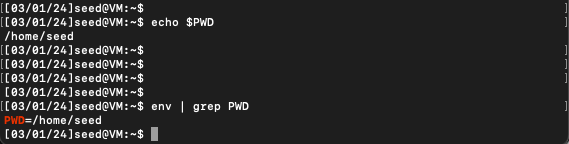
\includegraphics[width=0.35\textwidth]{figures/task1/task1.1.png}}
    \hfill
  \subfloat[set and unset env\label{fig:task1.2}]{%
        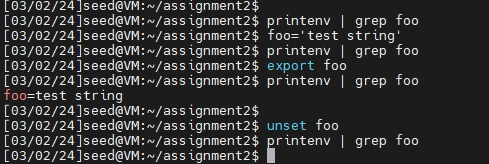
\includegraphics[width=0.54\textwidth]{figures/task1/task1.2.png}}
    \hfill
    \caption{Execute Result}\label{fig:task1}
\end{figure}

\textbf{Conclusion:}

Variables must be exported to appear in the environment. The `unset` command effectively removes them. This demonstrates the lifecycle of environment variables in Bash.

\subsection{Environment variable and Set-UID Programs}

Initially, \verb|foo| was unset and, as expected, didn't appear in the output of the Set-UID program. Upon setting \verb|foo| with a value but without exporting, \verb|foo| still did not show up. This is because the Set-UID program inherits only exported environment variables. After exporting \verb|foo|, it was then visible in the output, indicating that the Set-UID program did inherit \verb|foo| from the user's process as \ref{fig:task2}. 

\begin{figure}[h]
    \centering
       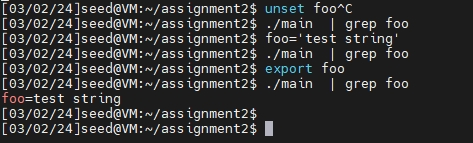
\includegraphics[width=0.7\textwidth]{figures/task2/task2.png}
    \caption{Execute Result}\label{fig:task2}
\end{figure}

\textbf{Conclusion:}

The Set-UID programs inherit exported environment variables from the user's process. This demonstrates how users can influence Set-UID program behavior through the environment, emphasizing the need for careful security practices around such programs.

\subsection{The PATH Environment variable and Set-UID Programs}

The manipulations with the \verb|PATH| variable and the Set-UID \verb|ls| program demonstrate how the system's behavior changed. Initially, the custom \verb|ls| program, when executed, listed the contents of the current directory, similar to the standard \verb|/bin/ls| command. After modifying the \verb|PATH| variable to include the current directory at the beginning and changing the ownership and permissions of the \verb|ls| program to mimic a Set-UID program, the \verb|ls| command should have executed the malicious program. However, the output indicates that the custom \verb|ls| program printed a message and the user IDs, which were both 1000, meaning it did not run with root privileges.

\begin{figure}[h]
    \centering
       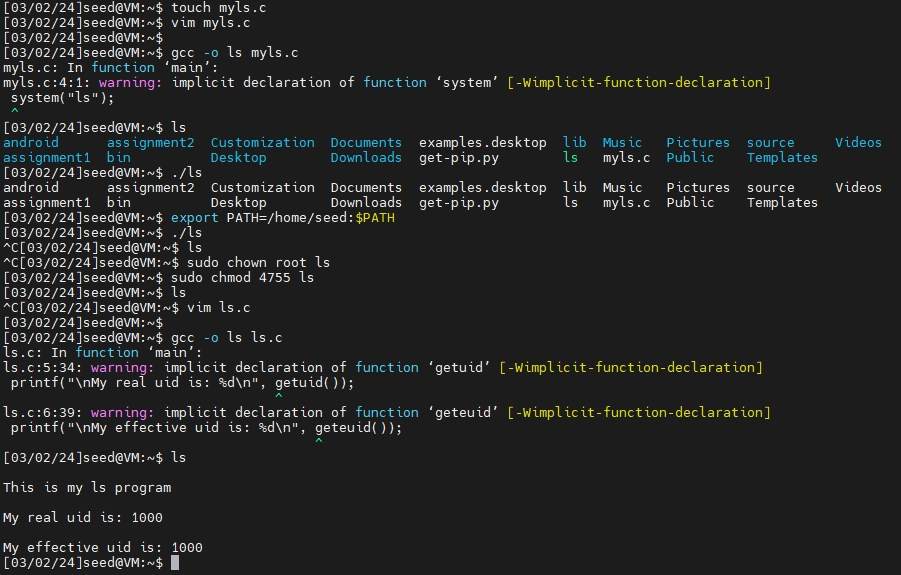
\includegraphics[width=0.95\textwidth]{figures/task3/task3.png}
    \caption{Execute Result}\label{fig:task3}
\end{figure}
\begin{figure}[h]
    \centering
       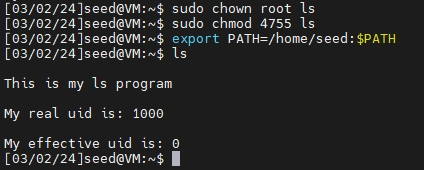
\includegraphics[width=0.5\textwidth]{figures/task3/task3.1.png}
    \caption{Execute Result After Set-UID}\label{fig:task3.1}
\end{figure}

\textbf{Conclusion:}

If the Set-UID program runs our code instead of the intended \verb|/bin/ls|, the code will execute with root privileges because Set-UID programs run with the effective permissions of the file owner, which is root in this case. This demonstrates a significant security risk with using relative paths in Set-UID programs and highlights the importance of using absolute paths for system calls.

\subsection{The LD\_PRELOAD environment variable and Set-UID Programs}
1. When \verb|myprog| was a regular program, running it as a normal user resulted in the overridden \verb|sleep| function being called, confirming that \verb|LD_PRELOAD| influenced the linker to load \verb|libmylib.so.1.0.1| first.

2. After making \verb|myprog| a Set-UID root program, running it as a normal user did not invoke the overridden \verb|sleep|, indicating that the Set-UID program did not inherit the \verb|LD_PRELOAD| variable from the user's environment, likely for security reasons.

3. Exporting \verb|LD_PRELOAD| in the root account and then running the Set-UID root \verb|myprog| resulted in the overridden \verb|sleep| being called, suggesting that when the Set-UID program is run by root, it respects the \verb|LD_PRELOAD| variable.

4. With \verb|myprog| set as a Set-UID program owned by another user (user1) and \verb|LD_PRELOAD| set in a non-root account, the overridden \verb|sleep| was not called, similar to the second case, reinforcing the idea that Set-UID programs ignore \verb|LD_PRELOAD| from non-owner environments.

\begin{figure}[h]
    \centering
       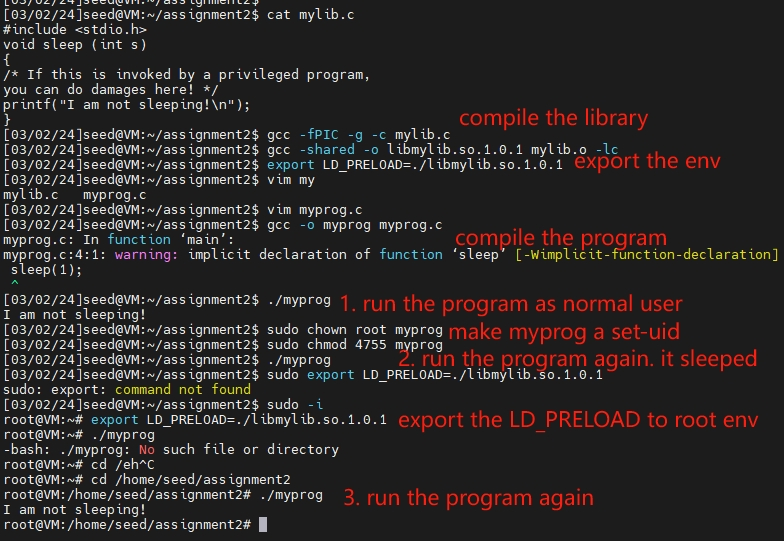
\includegraphics[width=0.9\textwidth]{figures/task4/task4.png}
    \caption{Execute Result}\label{fig:task4}
\end{figure}

\subsection{Invoking external programs using system() versus execve()}
1.If Bob were to exploit the \verb|system()| call with a command like ``./25 /etc/passwd; rm -f /path/to/some/file", as figured in \ref{fig:task5.1}, the shell would execute the \verb|cat /etc/passwd| command and then attempt the \verb|rm -f| command, potentially allowing unauthorized file deletion if the syntax were correct and the shell executes the second command.

The use of \verb|system()| in a Set-UID program poses a security risk due to its reliance on the shell, which can interpret additional commands and metacharacters. This risk is not present with \verb|execve()| as it does not invoke a shell and executes the specified command directly. The observations suggest that the program is functioning with elevated privileges, but the specific access to \verb|/etc/shadow| could not be confirmed from the provided output.

2.After recompiling and setting the program to use \verb|execve()|, any attempts to use command chaining or injection as part of the input to the Set-UID program should fail, as figured in \ref{fig:task5.2}, input such as \verb|filename; rm -f somefile| would not cause the deletion of \verb|somefile| because \verb|execve()| would attempt to pass the entire string as a single argument to \verb|/bin/cat|, which would then result in an error as it would be an invalid file name.
\begin{figure}[h]
    \centering
  \subfloat[Step 1 Execute Result\label{fig:task5.1}]{%
       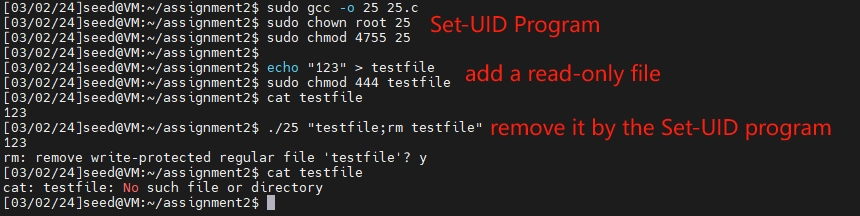
\includegraphics[width=0.95\textwidth]{figures/task5/task5.1.png}}
    \hfill
  \subfloat[Step 2 Execute Result\label{fig:task5.2}]{%
        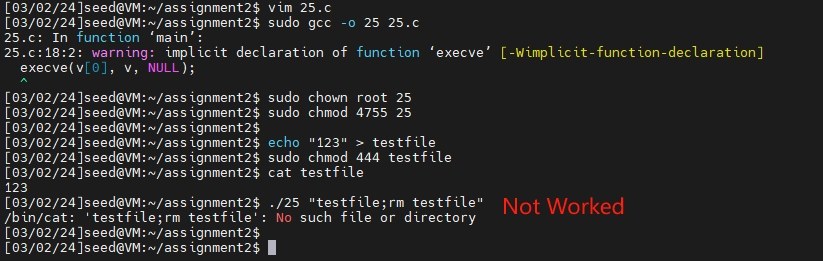
\includegraphics[width=0.95\textwidth]{figures/task5/task5.2.png}}
    \hfill
    \caption{Execute Result}\label{fig:task5}
\end{figure}



\subsection{Capability Leaking}
The program \verb|./26| successfully wrote "Malicious Data" to \verb|/etc/zzz|. Initially unable to open \verb|/etc/zzz|, after setting correct permissions and ownership, the Set-UID program, running with root privileges, opened \verb|/etc/zzz|. Upon dropping privileges with \verb|setuid(getuid())|, the child process inherited the file descriptor with root access, leading to the capability leak which allowed writing to the file, even as a non-privileged user. This demonstrates the security risk of inheriting file descriptors from privileged processes.

\begin{figure}[h]
    \centering
       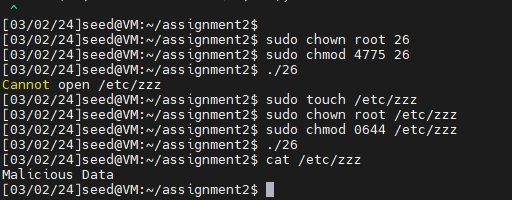
\includegraphics[width=0.7\textwidth]{figures/task6/task6.png}
    \caption{Execute Result}\label{fig:task6}
\end{figure}

\section{Buffer Overflow Vulnerability}

\subsection{Task 7: Programming using the Crypto Library}

\begin{lstlisting}[caption={find key script in Python},label={lst:task2.7},language=PYTHON,breaklines=true]
#!/usr/bin/python3
from Crypto.Cipher import AES
from Crypto.Util.Padding import pad

plaintext = "This is a top secret."
ciphertext = "764aa26b55a4da654df6b19e4bce00f4ed05e09346fb0e762583cb7da2ac93a2"
iv = "aabbccddeeff00998877665544332211"
plaindatabits = bytearray(plaintext, encoding='utf-8')
cipherdatabits = bytearray.fromhex(ciphertext)
ivdatabits = bytearray.fromhex(iv)

with open('./words.txt') as f:
  keys = f.readlines()

for k in keys:
  k = k.rstrip('\n')
  if len(k) <= 16:
    key = k + '#'*(16-len(k))
    cipher = AES.new(key=bytearray(key,encoding='utf-8'), mode=AES.MODE_CBC, iv=ivdatabits)
    testbits = cipher.encrypt(pad(plaindatabits, 16))
    if cipherdatabits == testbits:
      print("find the key:",key)
      exit(0)

print("cannot find the key!")
\end{lstlisting} 

The script use the Crypto to call the AES API in Python to encrypt the text, and simple loop to find a matched key in word list from a file.

After execute the script, the matched key is \textbf{``Syracuse"}.

\section{MD5 Collision Attack}
\subsection{Task 8: Generating Two Different Files with the Same MD5 Hash}
\begin{figure}[h]
    \centering
       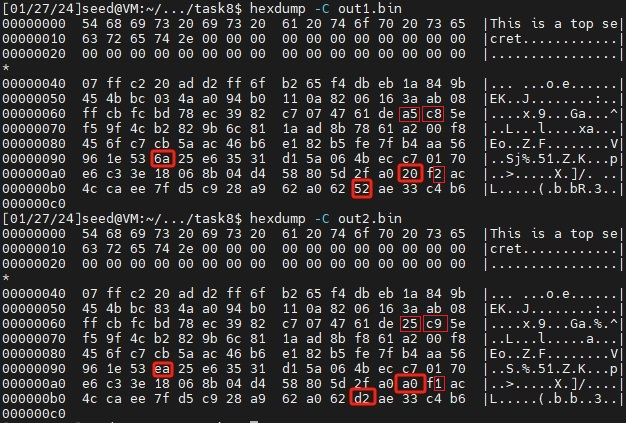
\includegraphics[width=0.6\textwidth]{figures/task8/md5coll.png}
    \caption{MD5 Collision}\label{fig:task8}
\end{figure}
\textbf{Question:}
\begin{enumerate}
    \item Length Not Multiple of 64: md5collgen might pad the prefix with additional bytes to reach a multiple of 64, as MD5 operates on 64-byte blocks.
    \item Prefix of Exactly 64 Bytes: No padding should be necessary, and the collision blocks will directly follow the prefix in both output files.
    \item Extent of Differences: The number and distribution of differing bytes can vary depending on the specific collision generated.
\end{enumerate}

\subsection{Task 9: Understanding MD5's Property}
\begin{lstlisting}[caption={MD5 Property test script},label={lst:task3.9},language=BASH,breaklines=true]
# out1.bin and out2.bin are  two files  generated in Task8 with the same MD5 hash:
$ md5sum out1.bin
189b839e730f57d79a8b4a98aadb36ea  out1.bin
$ md5sum out2.bin
189b839e730f57d79a8b4a98aadb36ea  out2.bin
# generate a suffix
$ echo -n "Lanch a missile." > suffix.txt
# concate two files with the suffix
$ cat out1.bin suffix.txt > out3.bin
$ cat out2.bin suffix.txt > out4.bin
# observe the concated files
$ md5sum out3.bin
30c758787b6e481692efd404ccb5c1a4  out3.bin
$ md5sum out4.bin
30c758787b6e481692efd404ccb5c1a4  out4.bin
\end{lstlisting} 

\textbf{Result:} 

The two concated files that with the same prefix MD5 and same suffix will result in the same result MD5 HASH value.

\subsection{Task 10: Generating Two Executable Files with the Same MD5 Hash}

\begin{lstlisting}[caption={MD5 Executable Program},label={lst:task3.10},language=BASH,breaklines=true]
# After Compliering the source code to Executable Program
# Cut the Executable Program to two parts
$ head -c 4224 out1 > prefix
$ tail -c +4287 out1 > suffix
# generated the same MD5 part of the program and join them to suffix
$ md5collgen -p prefix -o out1.bin out2.bin
$ cat out1.bin suffix > program1
$ cat out2.bin suffix > program2
# observe the MD5 of two Different program
$ md5sum program1
60824a7b99425740d90c0cfb41a34a1e  program1
$ md5sum program2
60824a7b99425740d90c0cfb41a34a1e  program2
$ chmod +x program1
$ chmod +x program2
$ ./program1
$ ./program2
# observe the execute result
\end{lstlisting} 

\begin{figure}[h]
    \centering
       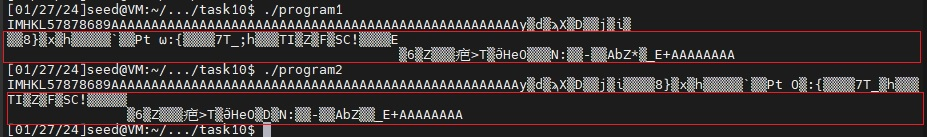
\includegraphics[width=0.96\textwidth]{figures/task10/executablefiles.png}
    \caption{Execute Result}\label{fig:task10}
\end{figure}

Obviously, they are not the same program according to the execute result but they have the same MD5 HASH value.

\subsection{Task 11: Making the Two Programs Behave Differently}

\begin{lstlisting}[caption={Different Behavior Program},label={lst:task3.11},language=BASH,breaklines=true]
# The same operation as TASK10
$ head -c 4160 program > prefix
$ md5collgen -p prefix -o out1.bin out2.bin
$ tail -c +4288 program > suffix
$ cat out1.bin suffix > test1
$ cat out2.bin suffix > test2
# Use bless modify both Y Array to be same as the X Array of test1
$ bless test1
$ bless test2
$ ./test1 # the X array and Y array are the same in test1
This is a good program
$ ./test2 # the X array and Y array are different in test2
This is a bad program
# Observe the MD5 HASH, they are the same
$ md5sum test1
8022e63d3dba85eb0ba3278ff78485c6  test1
$ md5sum test2
8022e63d3dba85eb0ba3278ff78485c6  test2
\end{lstlisting} 

\begin{figure}[h]
    \centering
       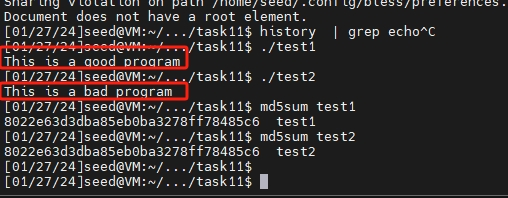
\includegraphics[width=0.96\textwidth]{figures/task11/differentbehaviors.png}
    \caption{Different Behavior}\label{fig:task11}
\end{figure}

\begin{figure}[h]
    \centering
  \subfloat[same arrays in test1\label{fig:task11test1}]{%
       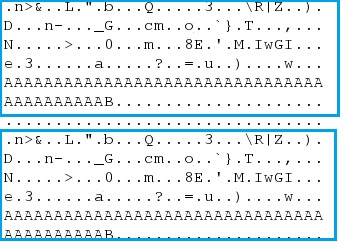
\includegraphics[width=0.48\textwidth]{figures/task11/test1.png}}
    \hfill
  \subfloat[different arrays in test2\label{fig:task11tes2}]{%
        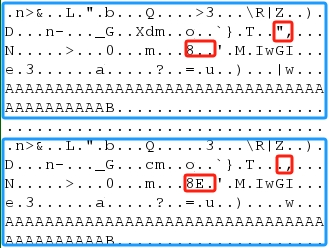
\includegraphics[width=0.48\textwidth]{figures/task11/test2.png}}
    \hfill
    \caption{test program binary}\label{fig:task11tests}
\end{figure}


\section{RSA Public-Key Encryption and Signature}

\subsection{BIGNUM APIs}
\subsection{A Complete Example}
The running example result is:
\begin{figure}[h]
    \centering
       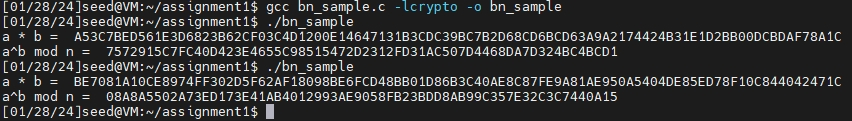
\includegraphics[width=0.96\textwidth]{figures/bignumresult.png}
    \caption{BIGNUM API Example}\label{fig:bignumexample}
\end{figure}

\subsection{Task 12: Deriving the Private Key}
\begin{lstlisting}[caption={C Program Code for Deriving the Private Key},label={lst:task4.12},language=C,breaklines=true]
#include <stdio.h>
#include <openssl/bn.h>
int main() {
    // Given values
    char p_hex[] = "F7E75FDC469067FFDC4E847C51F452DF";
    char q_hex[] = "E85CED54AF57E53E092113E62F436F4F";
    char e_hex[] = "0D88C3";
    // Convert hexadecimal strings to BIGNUM
    BIGNUM *p = BN_new();
    BIGNUM *q = BN_new();
    BIGNUM *e = BN_new();
    BN_hex2bn(&p, p_hex);
    BN_hex2bn(&q, q_hex);
    BN_hex2bn(&e, e_hex);
    // Calculate phi(n) = (p-1)*(q-1)
    BIGNUM *phi_n = BN_new();
    BN_sub(phi_n, p, BN_value_one());
    BN_sub_word(phi_n, 1);
    BN_mul(phi_n, phi_n, q, BN_CTX_new());
    BN_sub_word(phi_n, 1);
    // Calculate d = e^-1 mod phi(n)
    BIGNUM *d = BN_new();
    BN_mod_inverse(d, e, phi_n, BN_CTX_new());
    // Print the private key d
    char *d_hex = BN_bn2hex(d);
    printf("Private Key (d): %s\n", d_hex);
    // Free allocated memory
    return 0;
}
\end{lstlisting} 
\begin{lstlisting}[caption={Result of the Task 12},label={lst:task4.12-2},language=BASH,breaklines=true]
$ gcc main.c -lcrypto -o main
$ ./main
Private Key (d): 9B740D556F9080815E14B6633E9BCC3C87EAA0F0AD699E0A7E0719A725A94AA7
\end{lstlisting} 

\subsection{Task 13: Encrypting a Message}
\begin{lstlisting}[caption={C Program Code for Encrypt},label={lst:task4.13-1},language=C,breaklines=true]
#include <stdio.h>
#include <string.h>
#include <openssl/bn.h>
int main() {
    // Given public key values
    char n_hex[] = "DCBFFE3E51F62E09CE7032E2677A78946A849DC4CDDE3A4D0CB81629242FB1A5";
    char e_hex[] = "010001";
    // Given message
    char message_hex[] = "4120746f702073656372657421";  // Hex representation of "A top secret!"
    // Convert public key values to BIGNUM
    BIGNUM *n = BN_new();
    BIGNUM *e_value = BN_new();
    BN_hex2bn(&n, n_hex);
    BN_hex2bn(&e_value, e_hex);
    // Convert the message from hex to BIGNUM
    BIGNUM *message_bn = BN_new();
    BN_hex2bn(&message_bn, message_hex);
    // Allocate memory for the result
    BIGNUM *result = BN_new();
    // Perform encryption: ciphertext = message^e mod n
    BN_mod_exp(result, message_bn, e_value, n, BN_CTX_new());
    // Print the encrypted result
    char *result_hex = BN_bn2hex(result);
    printf("Encrypted Result: %s\n", result_hex);
    // Free allocated memory
    return 0;
}

\end{lstlisting}
\begin{lstlisting}[caption={C Program Code for Evaluation},label={lst:task4.13-2},language=C,breaklines=true]
#include <stdio.h>
#include <openssl/bn.h>
int main() {
    // Given private key values
    char n_hex[] = "DCBFFE3E51F62E09CE7032E2677A78946A849DC4CDDE3A4D0CB81629242FB1A5";
    char e_hex[] = "010001";
    char d_hex[] = "74D806F9F3A62BAE331FFE3F0A68AFE35B3D2E4794148AACBC26AA381CD7D30D";
    // Given ciphertext
    char ciphertext_hex[] = "6FB078DA550B2650832661E14F4F8D2CFAEF475A0DF3A75CACDC5DE5CFC5FADC";
    // Convert private key values to BIGNUM
    BIGNUM *n = BN_new();
    BIGNUM *e_value = BN_new();
    BIGNUM *d = BN_new();
    BN_hex2bn(&n, n_hex);
    BN_hex2bn(&e_value, e_hex);
    BN_hex2bn(&d, d_hex);
    // Convert ciphertext from hex to BIGNUM
    BIGNUM *ciphertext_bn = BN_new();
    BN_hex2bn(&ciphertext_bn, ciphertext_hex);
    // Allocate memory for the result
    BIGNUM *result = BN_new();
    // Perform decryption: message = ciphertext^d mod n
    BN_mod_exp(result, ciphertext_bn, d, n, BN_CTX_new());
    // Print the decrypted result
    char *result_hex = BN_bn2hex(result);
    printf("Decrypted Result: %s\n", result_hex);
    // Free allocated memory
    return 0;
}
\end{lstlisting} 

\begin{lstlisting}[caption={Result of the Task 13},label={lst:task4.13-3},language=BASH,breaklines=true]
$ ./main
Encrypted Result: 6FB078DA550B2650832661E14F4F8D2CFAEF475A0DF3A75CACDC5DE5CFC5FADC
$ ./decrypt
Decrypted Result: 4120746F702073656372657421
$ python -c 'print("4120746F702073656372657421".decode("hex"))'
A top secret!
\end{lstlisting} 

\subsection{Task 14: Decrypting a Message}
This Task is a lot of same with the Task 13. Just change the ciphertext value.

\begin{lstlisting}[caption={C Program Code for Decryption},label={lst:task4.14},language=C,breaklines=true]
//same with the Task 13 evaluation
#include <stdio.h>
#include <openssl/bn.h>
int main() {
    // Given private key values
    // Given ciphertext
    char ciphertext_hex[] = "8C0F971DF2F3672B28811407E2DABBE1DA0FEBBBDFC7DCB67396567EA1E2493F";
    // Convert private key values to BIGNUM
    //...
    // Free allocated memory
    return 0;
}
\end{lstlisting} 
\begin{lstlisting}[caption={Result of the Task 14},label={lst:task4.14-2},language=BASH,breaklines=true]
$ gcc decrypt.c -lcrypto -o decrypt
$ ./decrypt
Decrypted Result: 50617373776F72642069732064656573
$ python -c 'print("50617373776F72642069732064656573".decode("hex"))'
Password is dees
\end{lstlisting} 

\subsection{Task 15: Signing a Message}
Signature the message is using $S = m^d\ mod\ n$.
\begin{lstlisting}[caption={Result of the Task 15},label={lst:task15},language=BASH,breaklines=true]
$ python -c 'print("I owe you $2000.".encode("hex"))'
49206f776520796f752024323030302e # covert the text to hex
$ python -c 'print("I owe you $3000.".encode("hex"))'
49206f776520796f752024333030302e # covert the text to hex
$ gcc sign.c -lcrypto -o sign # sign.c is listing as Listing 20
$ ./sign
Signing: I owe you $2000.
Signature Result: 55A4E7F17F04CCFE2766E1EB32ADDBA890BBE92A6FBE2D785ED6E73CCB35E4CB
Signing: I owe you $3000.
Signature Result: BCC20FB7568E5D48E434C387C06A6025E90D29D848AF9C3EBAC0135D99305822
\end{lstlisting} 
\begin{lstlisting}[caption={C Program Code for Signature},label={lst:task4.15-2},language=C,breaklines=true]
#include <stdio.h>
#include <openssl/bn.h>
#include <string.h>
int main() {
    //signing the first message
    printf("Signing: I owe you $2000.\n");
    BIGNUM *m = BN_new();
    BN_hex2bn(&m, "49206f776520796f752024323030302e");
    BIGNUM *d = BN_new();
    BIGNUM *n = BN_new();
    BN_hex2bn(&d, "74D806F9F3A62BAE331FFE3F0A68AFE35B3D2E4794148AACBC26AA381CD7D30D");
    BN_hex2bn(&n, "DCBFFE3E51F62E09CE7032E2677A78946A849DC4CDDE3A4D0CB81629242FB1A5");
    BIGNUM *signature = BN_new();
    //s = m ^ d mod n
    BN_mod_exp(signature, m, d, n, BN_CTX_new());
    char *signature_hex = BN_bn2hex(signature);
    printf("Signature Result: %s\n", signature_hex);
    //signing another message
    printf("Signing: I owe you $3000.\n");
    BIGNUM *m2 = BN_new();
    BN_hex2bn(&m2, "49206f776520796f752024333030302e");
    BN_mod_exp(signature, m2, d, n, BN_CTX_new());
    //...
    // Free BIGNUMs
    return 0;
}
\end{lstlisting} 
\textbf{Compare both signatures}, obviously the message has only 1 bit change while the signature is totally different.

\subsection{Task 16: Verifying a Message}
Signature the message is using $m' = s^e\ mod\ n$. And then compare the whether $m' = m?$
\begin{lstlisting}[caption={C Program Code for Verifying},label={lst:task4.16},language=C,breaklines=true]
#include <stdio.h>
#include <openssl/bn.h>
#include <string.h>
int main() {
    // Convert signature to BIGNUM
    BIGNUM *signature = BN_new();
    BN_hex2bn(&signature, "643D6F34902D9C7EC90CB0B2BCA36C47FA37165C0005CAB026C0542CBDB6802F");
    // Encrypt the message using Alice's public key
    BIGNUM *e = BN_new();
    BIGNUM *n = BN_new();
    BIGNUM *message = BN_new();
    BN_hex2bn(&e, "010001");
    BN_hex2bn(&n, "AE1CD4DC432798D933779FBD46C6E1247F0CF1233595113AA51B450F18116115");
    BN_hex2bn(&message, "4c61756e63682061206d697373696c652e");
    BIGNUM *test_message = BN_new();
    //m' = s ^ e mod n
    BN_mod_exp(test_message, signature, e, n, BN_CTX_new());
    // Compare the m with m'
    if (BN_cmp(message, test_message) == 0) {
        printf("Signature is valid.\n");
    } else {
        printf("Signature is invalid.\n");
    }
    // Free BIGNUMs
}
\end{lstlisting} 
\begin{figure}[h]
    \centering
       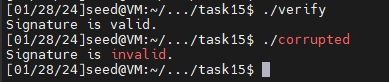
\includegraphics[width=0.5\textwidth]{figures/task16/messageverify.png}
    \caption{Verification Result}\label{fig:task16}
\end{figure}
Figure \ref{fig:task16} show the result of the right signature and  the corrupted one, respectively. 

The modified signature (with 3F) won't match the encrypted message generated using Alice's public key. 

And RSA signature verification is highly sensitive to even minor changes in the signature or message.

\subsection{Task 17: Manually Verifying an X.509 Certificate}
According to Step 1 to Step 4, the X.509 certificate detailed is:
\begin{figure}[h]
    \centering
  \subfloat[Modulus]{%
       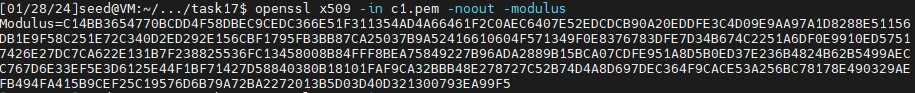
\includegraphics[width=0.9\textwidth]{figures/task17/m.png}}
    \hfill
  \subfloat[Exponent]{%
        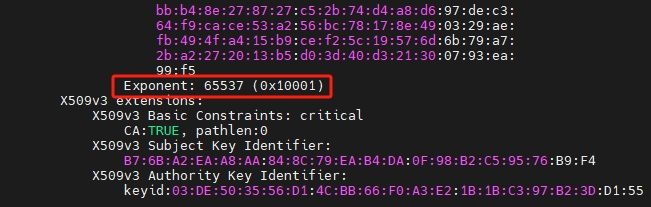
\includegraphics[width=0.45\textwidth]{figures/task17/e.png}}
    \hfill
  \subfloat[Signature]{%
        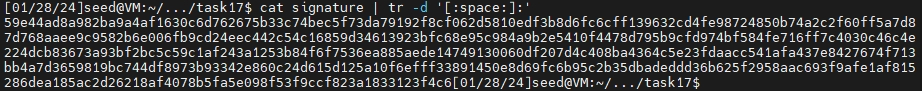
\includegraphics[width=0.9\textwidth]{figures/task17/s.png}}
    \hfill
  \subfloat[Body HASH]{%
        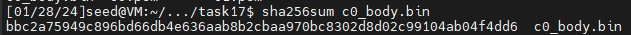
\includegraphics[width=0.8\textwidth]{figures/task17/h.png}}
    \hfill
    \caption{Task 17 Information}\label{fig:task17}
\end{figure}

And then, a program to verity the information as follows:
\begin{lstlisting}[caption={C Program Code for Manually Verifying},label={lst:task17},language=C,breaklines=true]
#include <stdio.h>
#include <openssl/bn.h>
#include <string.h>
int main()
{
    char bodyhash[] = "BBC2A75949C896BD66DB4E...302D8D02C99104AB04F4DD6"; # the Body HASH
    BIGNUM *n = BN_new();
    BIGNUM *e = BN_new();
    BIGNUM *s = BN_new();
    BIGNUM *m = BN_new();
    BN_hex2bn(&n, "C14BB3654770BC...F5"); # the Modulus
    BN_hex2bn(&e, "010001"); # the Exponent
    BN_hex2bn(&s, "59e44ad8a982ba9a4af163...23f4c6"); # the Signature
    BN_mod_exp(m, s, e, n, BN_CTX_new());
    char *message_hex = BN_bn2hex(m);
    size_t length = strlen(message_hex);
    //compare the last 64 bytes
    if (length > 64) {
        // Move the pointer to the start of the last 64 bytes
        char *substring = message_hex + (length - 64);
        // Print or manipulate the substring as needed
        int result = strcmp(substring, bodyhash);
        if (result == 0) {
            printf("Verification PASS.\n");
        } else {
            printf("Verification Failed\n");
        }
    } else {
        // If the string is shorter than 64 bytes, handle it accordingly
        printf("Something Wrong");
    }
    return 0;
}
\end{lstlisting} 
\begin{figure}[h]
    \centering
       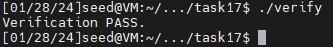
\includegraphics[width=0.4\textwidth]{figures/task17/result.png}
    \caption{Verification Result}\label{fig:task17result}
\end{figure}
\section{Pseudo Random Number Generation}
\subsection{Task 18: Generate Encryption Key in a Wrong Way}
\begin{figure}[h]
    \centering
       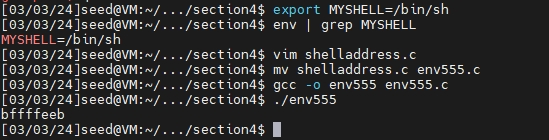
\includegraphics[width=0.6\textwidth]{figures/task18/task18.png}
    \caption{Result Observation}\label{fig:task18result}
\end{figure}

The \verb|time(NULL)| function returns the current time as the number of seconds since the Epoch (1970-01-01 00:00:00 +0000 UTC). It prints this value to the console.

\verb|srand(time(NULL))| seeds the pseudo-random number generator \verb|(rand())| with the current time. The purpose of seeding is to initialize the random number generator with a somewhat unpredictable value, ensuring that subsequent calls to rand() produce different sequences of pseudo-random numbers.

When comment out the line \verb|srand(time(NULL))| (Line 13) and rerun the program, the pseudo-random numbers generated by \verb|rand()| will be the same every time when running the program because the generator is not reseeded. 

In summary, the \verb|srand(time(NULL))| line is responsible for seeding the pseudo-random number generator based on the current time, introducing unpredictability and ensuring a different sequence of pseudo-random numbers each time the program is executed.

\subsection{Task 19: Guessing the Key}
Firstly, I program a C program to generate all potential key from time to time accordingly.
\begin{lstlisting}[caption={C Program Code for Generating Keys},label={lst:task19-1},language=C,breaklines=true]
#include <stdio.h>
#include <stdlib.h>
#include <time.h>
#define KEYSIZE 16
void main() {
    long long int timestamp;
    for(timestamp = 1523920129; timestamp <= 1523920129+2*24*60*60; timestamp++) {
        char key[KEYSIZE];
        srand(timestamp);
        for (int i = 0; i< KEYSIZE; i++){
            key[i] = rand()%256;
            printf("%.2x", (unsigned char)key[i]);
        }
        printf("\n");
    }
}
\end{lstlisting} 

And using \verb|genkey > key.txt| to generate a key files, after generating, then I use a Python script to find the key.
\begin{lstlisting}[caption={Python Script for Finding the Key},label={lst:task19-2},language=PYTHON,breaklines=true]
import binascii
from Crypto.Cipher import AES
# Read keys from the file
with open('./key.txt') as fp:
    keys = fp.readlines()
# Iterate through each key in the file
for keyhex in keys:
    # Remove trailing newline characters
    keyhex = keyhex.rstrip()
    # Convert IV, key, and plaintext from hex to bytes
    iv = binascii.unhexlify('09080706050403020100A2B2C2D2E2F2'.lower())
    key = binascii.unhexlify(keyhex.lower())
    plaintext = binascii.unhexlify('255044462d312e350a25d0d4c5d80a34'.lower())
    # Create AES encryptor object
    encryptor = AES.new(key, AES.MODE_CBC, iv)
    # Encrypt the plaintext
    ciphertext = encryptor.encrypt(plaintext)
    # Check if the ciphertext matches the known value
    if ciphertext == binascii.unhexlify('d06bf9d0dab8e8ef880660d2af65aa82'.lower()):
        print("Key Found: " + binascii.hexlify(key))
\end{lstlisting} 
\begin{figure}[h]
    \centering
       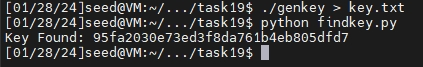
\includegraphics[width=0.6\textwidth]{figures/task19/result.png}
    \caption{Result}\label{fig:task19result}
\end{figure}
And finally find the key: \verb|95fa2030e73ed3f8da761b4eb805dfd7|

\subsection{Task 20: Measure the Entropy of Kernel}
Since my Seed lab is running in a remote VM, I try to measure the entropy by such:
\begin{itemize}
    \item User input:
    Typing rapidly and randomly on the keyboard introduces unpredictable timing between key presses, boosting entropy.
    \item Moving the mouse remotely in X11 erratically and clicking randomly generates unpredictable mouse events, adding to entropy.
    \item Disk activity:
    Reading large files from a hard drive or SSD creates variable disk access times due to seek times and read speeds, contributing to entropy.
    \item Network activity:
    Visiting the server by ssh involves network interactions that introduce variability in packet arrival times and server responses, increasing entropy.
    Downloading large files also involves unpredictable network delays and data transfer patterns.
\end{itemize}
These activities significantly increase entropy.
\begin{figure}[h]
    \centering
  \subfloat[Background Entropy]{%
       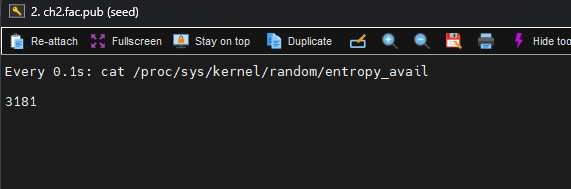
\includegraphics[width=0.45\textwidth]{figures/task20/watch1.png}}
    \hfill
  \subfloat[Activity Entropy]{%
        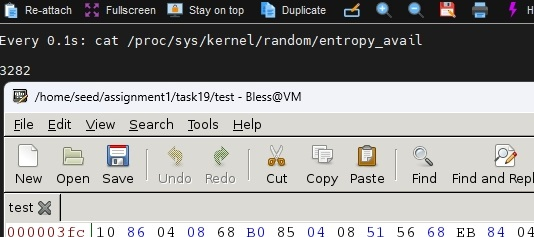
\includegraphics[width=0.4\textwidth]{figures/task20/watch2.png}}
    \hfill
    \caption{Task 20 Observation}\label{fig:task20}
\end{figure}

\subsection{Task 21: Get Pseudo Random Numbers from /dev/random}
In the task, when execute the command, \verb!cat /dev/random | hexdump!, the entropy will decrease significantly, when the entropy approaching 0, the command will stop outputing any information. 
And I try to increase the entropy by upload a file to the server, shown as \ref{fig:task21}(b),
\begin{figure}[h]
    \centering
  \subfloat[Background Entropy]{%
       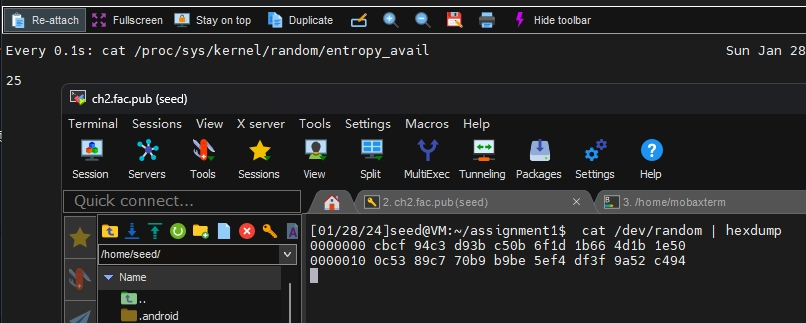
\includegraphics[width=0.45\textwidth]{figures/task21/watch1.png}}
    \hfill
  \subfloat[Upload a file for increasign the Entropy]{%
        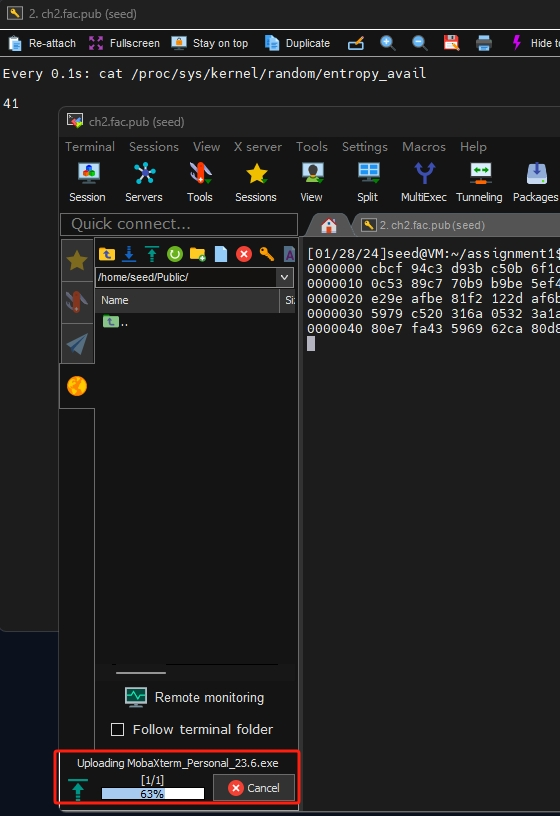
\includegraphics[width=0.4\textwidth]{figures/task21/watch2.png}}
    \hfill
    \caption{Task 21 Observation}\label{fig:task21}
\end{figure}

\textbf{Q: Launching a DoS Attack:}

\textbf{Exhaust Entropy Pool:}
Flood the server with requests that require random numbers from \verb|/dev/random|.
This depletes the entropy pool faster than it can be replenished, causing \verb|/dev/random| to block.

\textbf{Prevent Entropy Refilling:}
Avoid activities that generate entropy, like mouse movements, keyboard input, or disk I/O.
This prevents the server from replenishing the entropy pool and resuming normal operations.

\textbf{Impact:}
The server will become unresponsive to new requests that require random numbers, effectively denying service.

\textbf{Prevention:}
Use \verb|/dev/urandom| for non-critical randomness: \verb|/dev/urandom| doesn't block and is suitable for most applications.
Consider hardware RNGs: Hardware random number generators provide a more resilient source of entropy.
Implement rate limiting: Restrict the rate of requests that use \verb|/dev/random| to mitigate depletion attacks.
Monitor entropy levels: Set up alerts for low entropy conditions to allow for proactive measures.

\subsection{Task 22: Get Random Numbers from /dev/urandom}

\begin{figure}[h]
    \centering
       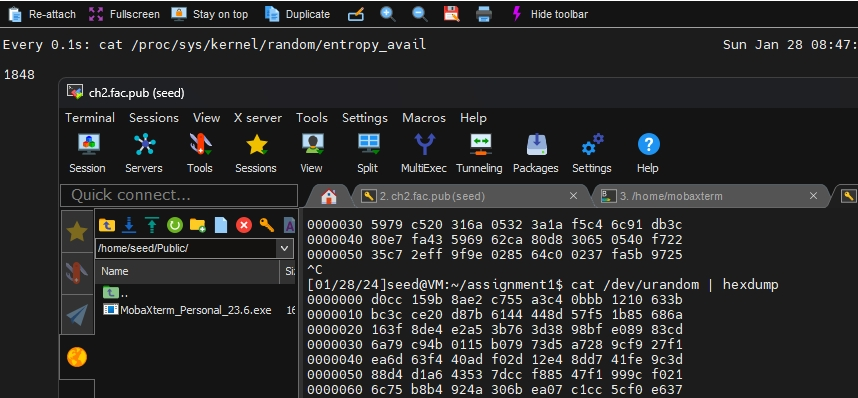
\includegraphics[width=0.6\textwidth]{figures/task22/watch1.png}
    \caption{Not block random number generating by /dev/urandom}\label{fig:task22observation-1}
\end{figure}

\begin{figure}[h]
    \centering
       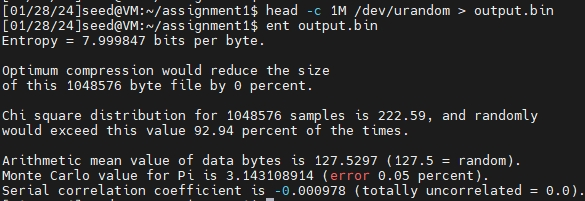
\includegraphics[width=0.6\textwidth]{figures/task22/watch2.png}
    \caption{Measurement of the random number generating by /dev/urandom}\label{fig:task22observation-2}
\end{figure}

Behavior of \verb|/dev/urandom|:

\textbf{No blocking:} Unlike \verb|/dev/random|, \verb|/dev/urandom| won't block, even when the entropy pool is low. It will continue generating pseudorandom numbers using the available seed.

\textbf{Network workload:} won't have a noticeable effect on the output of \verb!cat /dev/urandom | hexdump!. This is because \verb|/dev/urandom| doesn't directly rely on real-time entropy input.

\textbf{Quality of Random Numbers:}
Testing with ent: The ent tool evaluates randomness based on statistical tests. Good results typically indicate: Entropy estimates close to 8 bits per byte.

Passing most or all statistical tests.
No significant patterns or correlations in the data.

\begin{lstlisting}[caption={C Program Code for Generating Keys by /dev/urandom},label={lst:task22},language=C,breaklines=true]
#include <stdio.h>
#include <stdlib.h>
#define KEY_LEN 32  // 256 bits
int main() {
    unsigned char *key = (unsigned char *)malloc(sizeof(unsigned char) * KEY_LEN);
    FILE *random = fopen("/dev/urandom", "r");
    if (random == NULL) {
        perror("Error opening /dev/urandom");
        return 1;
    }
    fread(key, sizeof(unsigned char) * KEY_LEN, 1, random);
    fclose(random);
    // Print the generated key (replace with secure handling for actual use):
    printf("Generated 256-bit encryption key: ");
    for (int i = 0; i < KEY_LEN; i++) {
        printf("%02x", key[i]);
    }
    printf("\n");
    free(key);
    return 0;
}

\end{lstlisting} 

\begin{figure}[h]
    \centering
       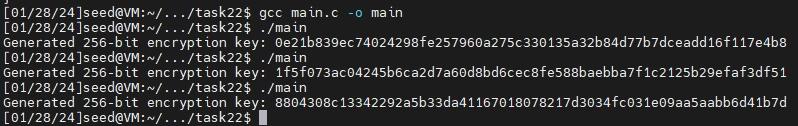
\includegraphics[width=0.9\textwidth]{figures/task22/watch3.png}
    \caption{Generating Key by /dev/urandom}\label{fig:task22observation-3}
\end{figure}
This code generates a 256-bit encryption key using \verb|/dev/urandom|. It allocates memory for the key, opens \verb|/dev/urandom|, reads random bytes into the key, prints the key in hexadecimal format, and then frees the allocated memory. Compile and run this code to obtain your 256-bit encryption key.

%------------------------------------------------

%\bibliographystyle{ieeetr}
%\bibliography{references} % citation records are in the references.bib document

\end{document}
